% Template for ISBI-2008 paper; to be used with:
%          spconf.sty  - ICASSP/ICIP LaTeX style file, and
%          IEEEbib.bst - IEEE bibliography style file.
% --------------------------------------------------------------------------
\documentclass[a4paper, oneside, 12pt, onecolumn]{article}
\usepackage{amsmath,amssymb,graphicx,dsfont,setspace}

% Example definitions.
% --------------------
\def\x{{\mathbf x}}
\def\L{{\cal L}}
\def\M{{\mathcal M}}

% Title.
% ------
\title{Analysis on brain catalogue data}
%
% Single address.
% ---------------
%\author{Julien Lef\`evre}
\date{May 24, 2016}

%
% For example:
% ------------
%\address{School\\
%   Department\\
%   Address}
%
% Two addresses (uncomment and modify for two-address case).
% ----------------------------------------------------------
%\twoauthors
%  {A. Author-one, B. Author-two\sthanks{Thanks to XYZ agency for funding.}}
%   {School A-B\\
%   Department A-B\\
%   Address A-B}
%  {C. Author-three, D. Author-four\sthanks{The fourth author performed the work
%   while at ...}}
%   {School C-D\\
%   Department C-D\\
%   Address C-D}
%
\begin{document}
%\ninept
%
\maketitle
%
%\doublespacing

\section{Curvedness and shape index}

Curvedness and shape index are quantities derived from local curvatures of a 2D surface \cite{koenderink1987representation}. Similarly to mean curvature or gaussian curvature, they offer a bivariate representation of the local geometry.\\
The curvedness is a positive value that represents the amplitude of the folding. The value $0$ corresponds to a locally flat surface. The shape index is a \emph{scale-invariant} value between $-1$ and $1$. $-1$ is a pit, $-1/2$ an archetypal sulcus, $0$ a saddle, $1/2$ an archetypal gyrus and $1$ a calotte. Fig \ref{Fig1} shows different surfaces associated to different points in the shape index/curvedness space.\\

\begin{figure}
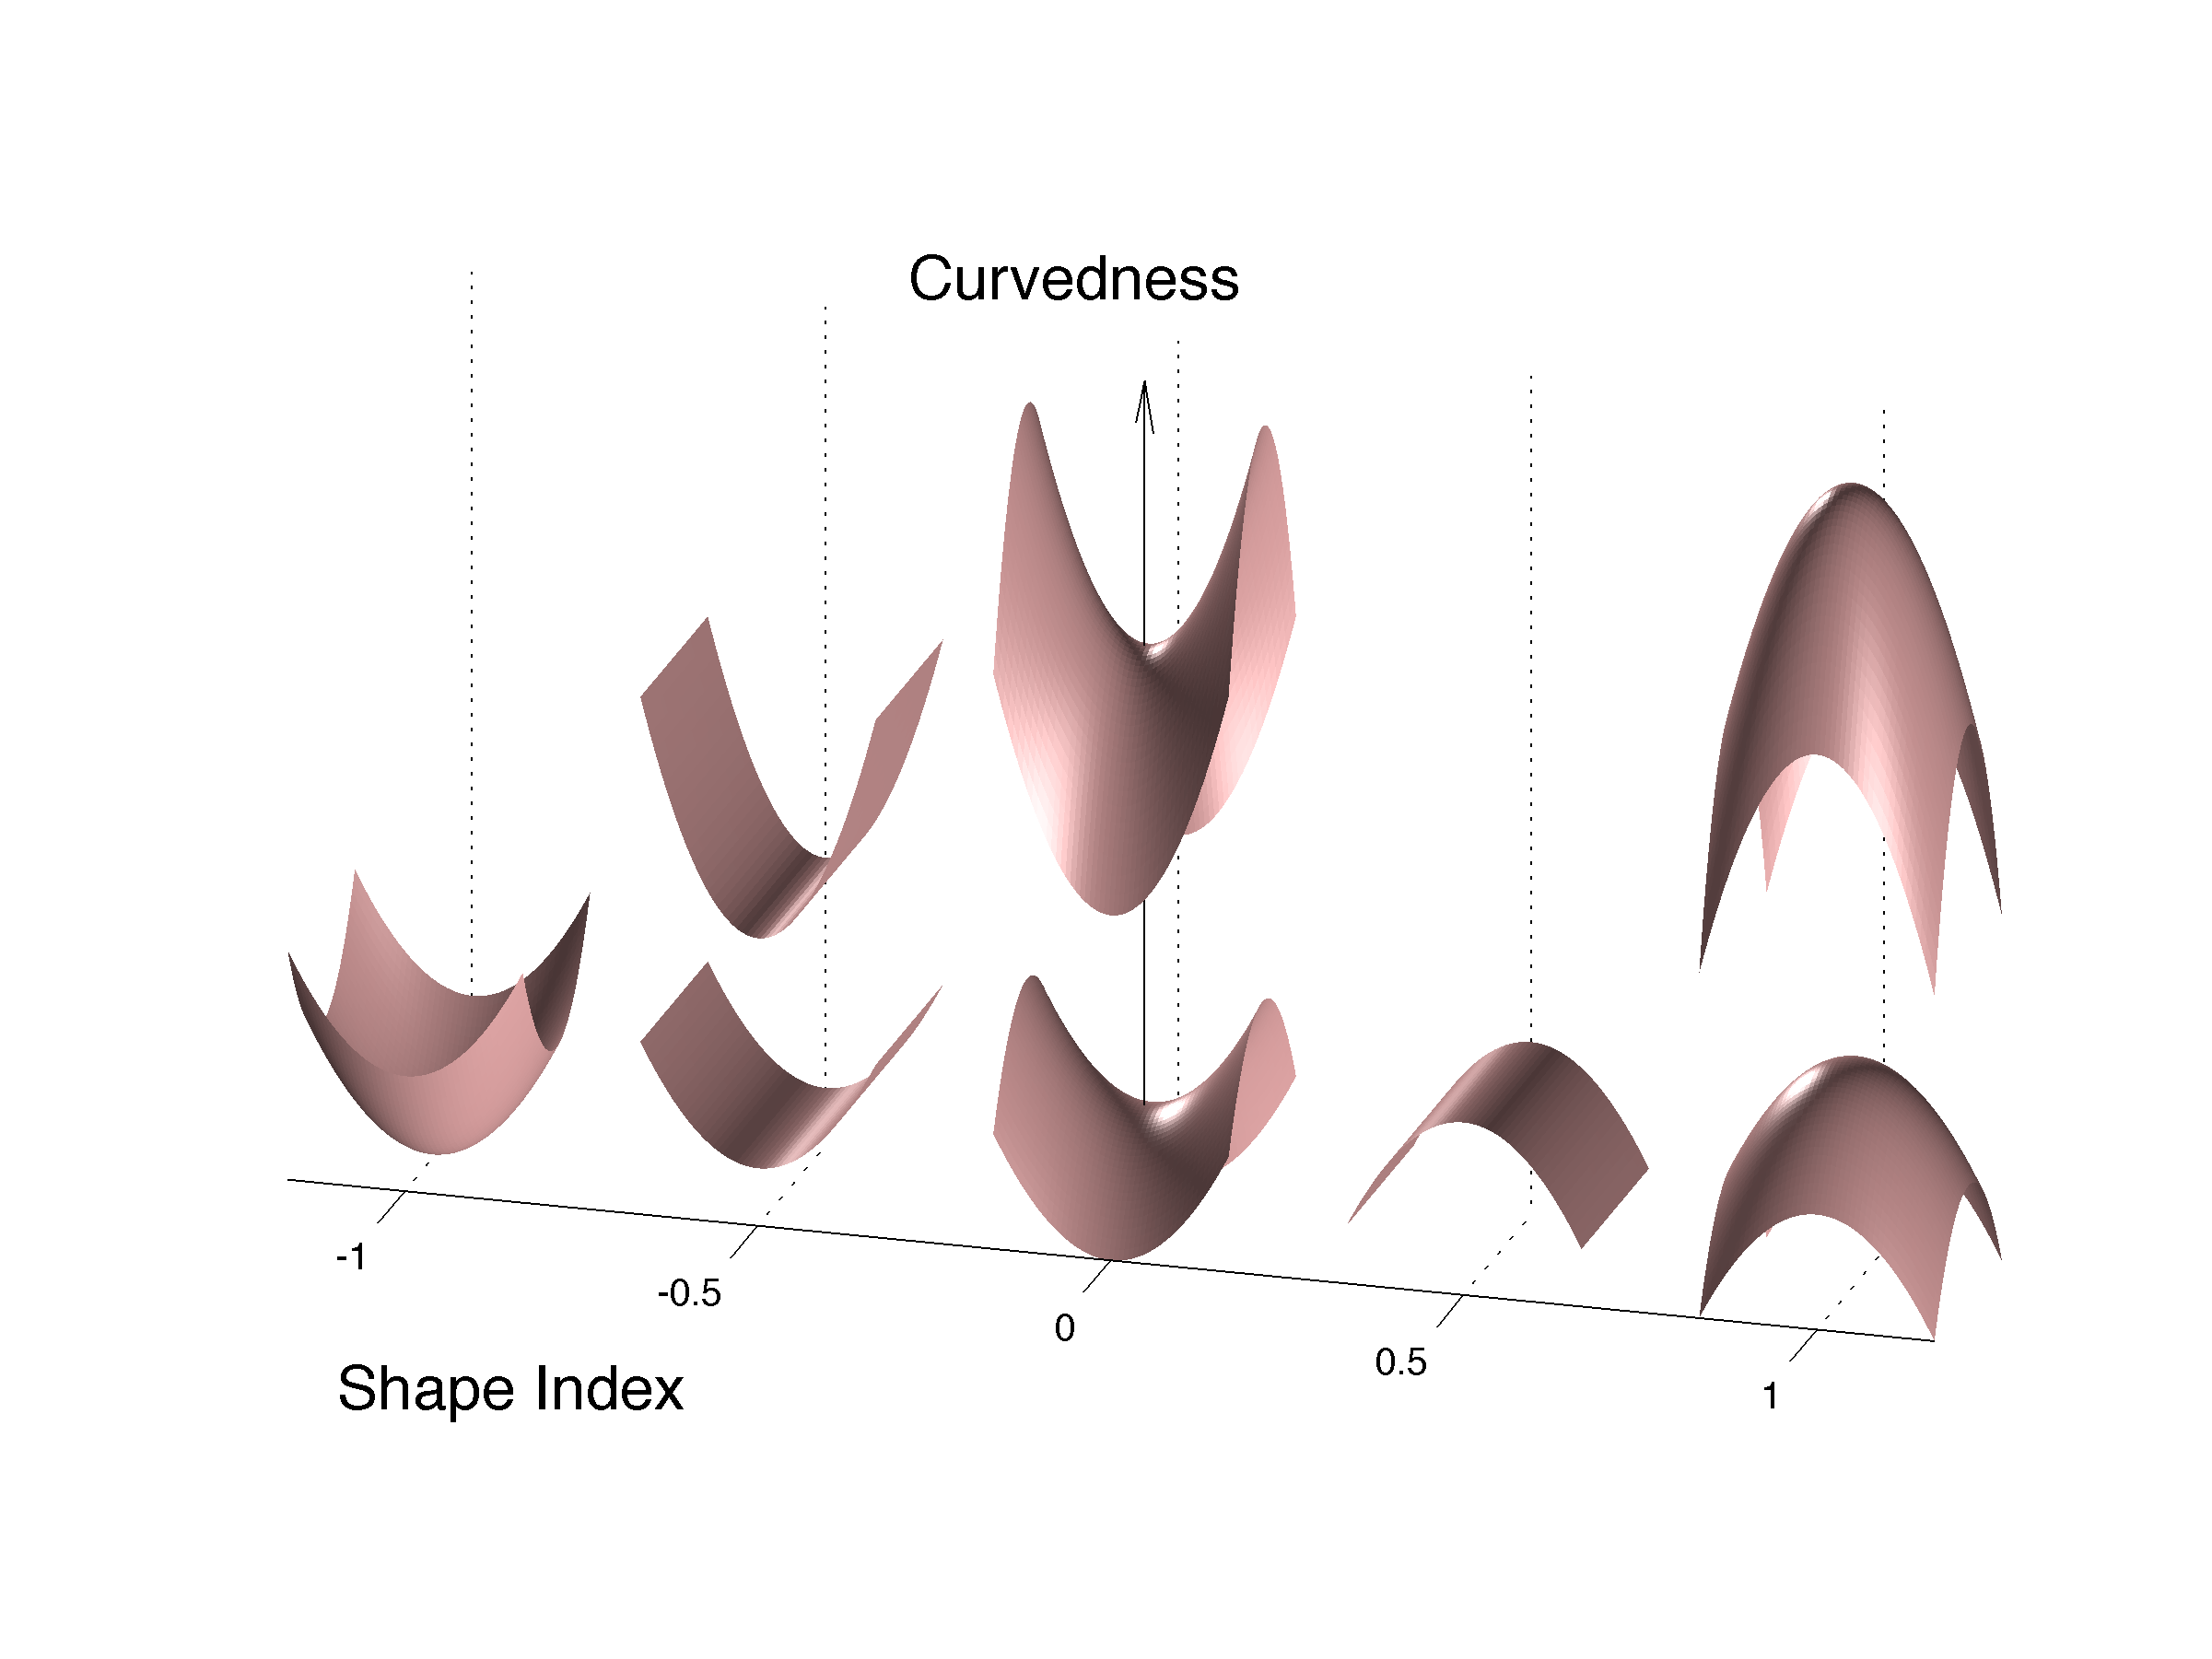
\includegraphics[width=\linewidth]{Figs/SI_C_scheme.png}
\caption{Illustration of curvedness and shape index on different local geometries.}
\label{Fig1}
\end{figure}

Curvedness and shape index are computed by obtaining first the principal curvatures at each vertex of the mesh with the function \texttt{principal\_curvature} and secondly with the function \texttt{curvedness\_shape}.

\section{Spherical parameterization}

A relatively simple and fast method to parameterize (brain) surfaces has been proposed in \cite{lefevre2015spherical}. It is based on the first eigenfunctions of the Laplace-Beltrami Operator that can be visualized as images on a surface (see Fig \ref{Fig2}). Those eigenfunctions represent low-frequency modes of oscillation of the surface. They correspond to $\cos$ and $\sin$ functions for more general domains than a 1D segment.\\

\begin{figure}
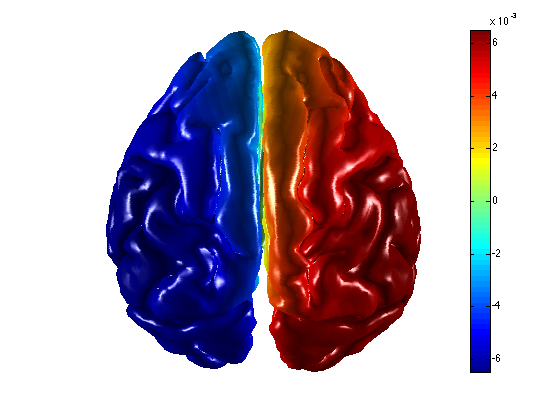
\includegraphics[width=0.32\linewidth]{Figs/orang_VP1.png}
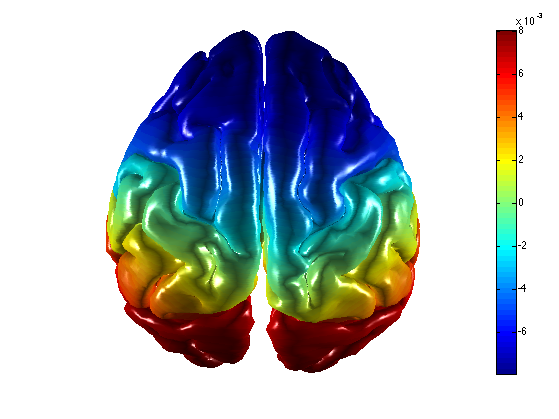
\includegraphics[width=0.32\linewidth]{Figs/orang_VP2.png}
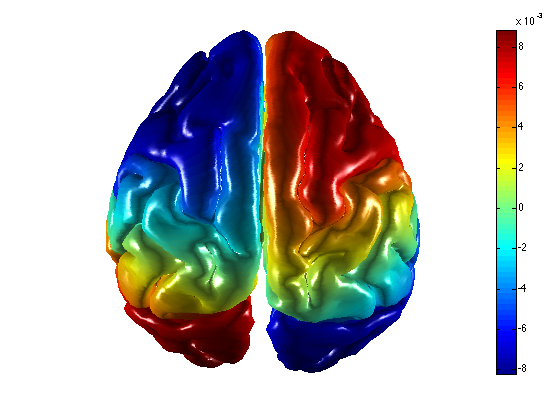
\includegraphics[width=0.32\linewidth]{Figs/orang_VP3.png}
\caption{3 first eigenfunctions of the Laplace-Beltrami Operator.}
\label{Fig2}
\end{figure}

An important notion for the parameterization method is to define \emph{nodal domains}. Nodal domains of an eigenfunction correspond to subregions of a mesh where the eigenfunction has a constant sign. A fundamental theorem due to Courant says that the eigenfunction of order $n$ cannot have more than $n+1$ nodal domains. It is verified on Fig \ref{Fig2} where we can observe that eigenfunctions 1, 2 and 3 have respectively 2, 2 and 4 nodal domains.\\
In \cite{lefevre2015spherical} a conjecture has been proposed to build a natural transformation from a closed mesh onto the sphere by using the three first eigenfunctions, \emph{provided that they have only 2 nodal domains}. In the example of Fig \ref{Fig2} the third eigenfunction has not the required property so we can use the fourth eigenfunction to satisfy the conditions of the conjectural theorem (see Fig \ref{Fig3}). Note that in the general case, there are no guarantees that there could exist at least 3 eigenfunctions with 2 nodal domains (it might be a reasonable conjecture).\\

\begin{figure}
\center
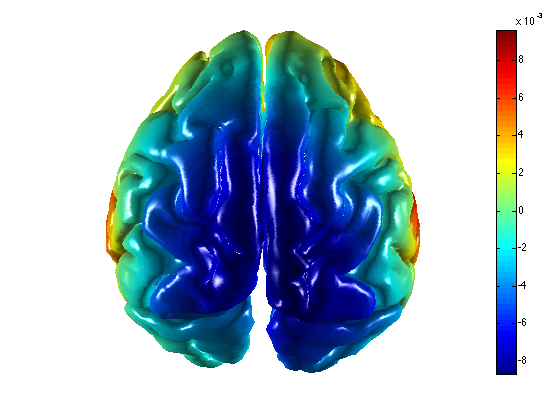
\includegraphics[width=0.32\linewidth]{Figs/orang_VP4_1.png}
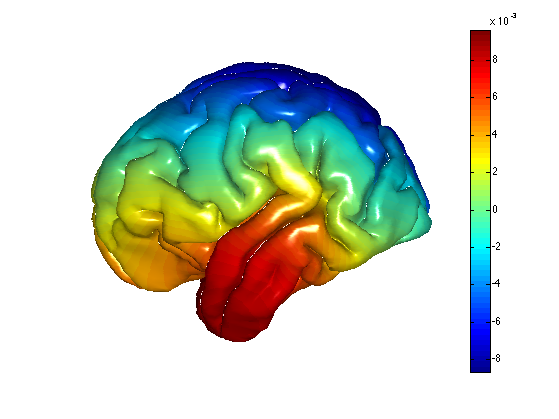
\includegraphics[width=0.32\linewidth]{Figs/orang_VP4_2.png}
\caption{Fourth eigenfunction of the Laplace-Beltrami Operator through 2 different views.}
\label{Fig3}
\end{figure}

The Laplace-Beltrami eigenfunctions are computed by using two sparse matrices obtained from geometric characteristics of the mesh, through the functions \texttt{heat\_matrices} and \texttt{eigs}. Then the spherical mapping is achieved with the function \texttt{map2sphere}.

\section{Group analysis}

In the perspective of doing group analysis across species, it is important 1) to define a local metric of interest (surface ratio, local gyrification index, curvature-based quantities....) 2) that can be compared across surfaces by using a registration method.\\

The two previous sections offer two ingredients for doing a group analysis but it remains to define the pointwise correspondence between two surfaces. The spherical parameterization defined previously is one possibility amon many other spherical parameterization methods (Freesurfer, HIPHOP....) and surface registration method (Deformetrika....). The idea is to resample a map defined on a spherical mesh that parameterizes an individual surface onto another spherical mesh which can be a template sphere or another spherical mesh (in the perspective of pairwise comparison). For that we use the function \texttt{tex\_to\_mesh\_SD} which calls \texttt{MARS\_linearInterpolate} and other functions of the spherical demons toolbox.\\

\begin{figure}
\center
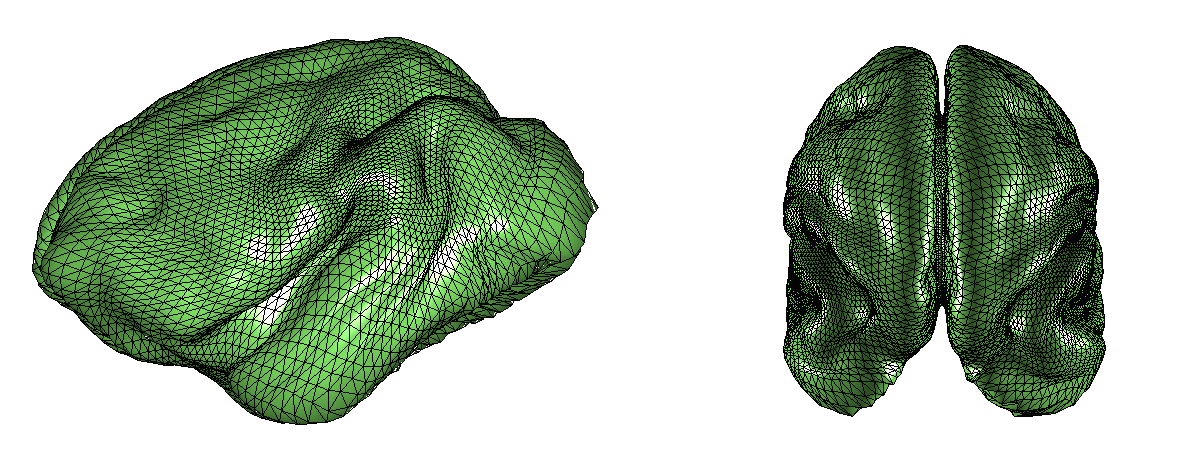
\includegraphics[width=0.6\linewidth]{Figs/mean_shape.png}
\caption{Average brain. The underlying regular meshing used for the sphere is represented in black.}
\label{Fig4}
\end{figure}

It is possible to resample the coordinates of each individual surface and to compute an average of each coordinates. This procedure is quite common when it comes to do group analysis on a homogeneous populations but is probably less relevant here, because of the dramatic changes in terms of folding between small and large brains (see Fig \ref{Fig4}).\\

\begin{figure}
\center
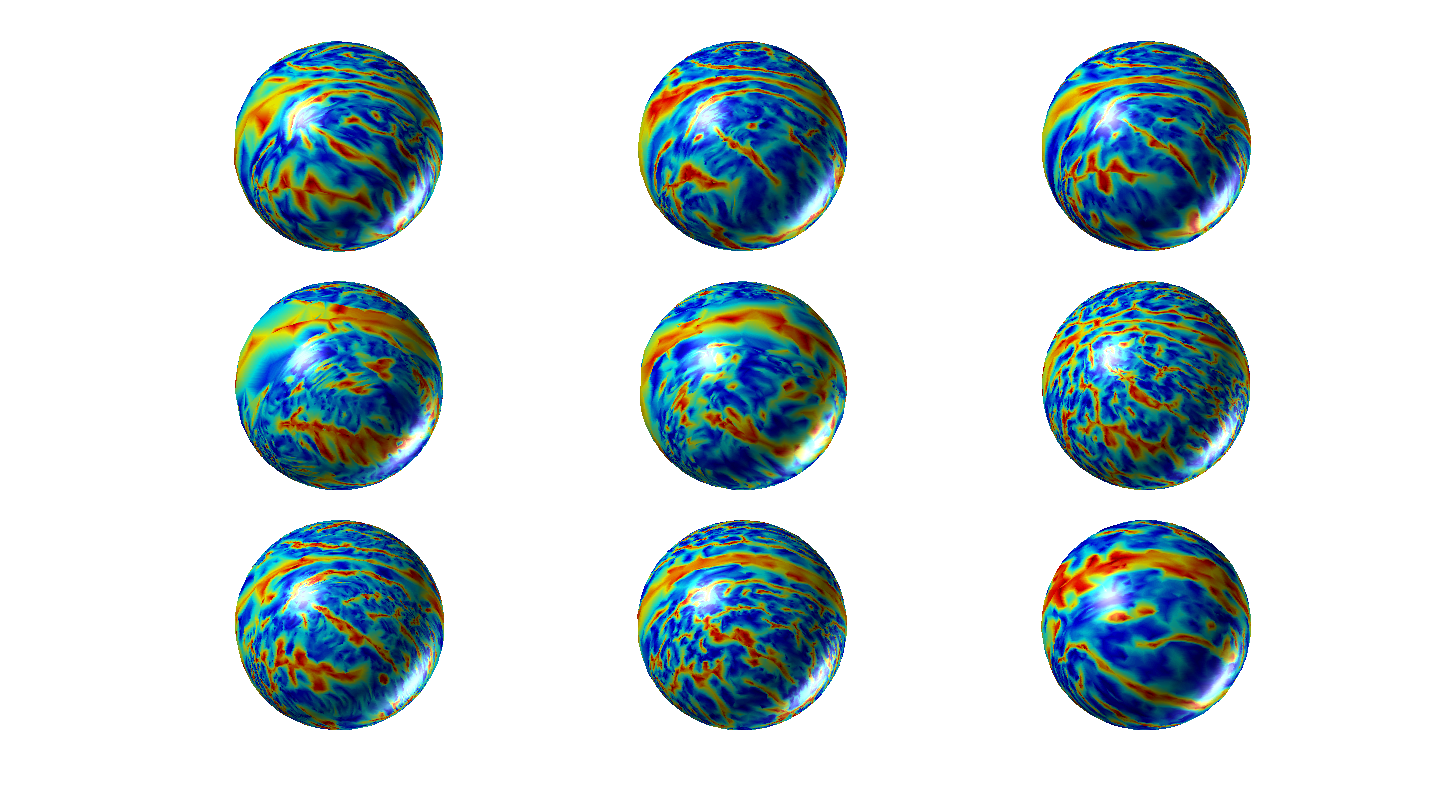
\includegraphics[width=0.45\linewidth]{Figs/all_both_SI.png}
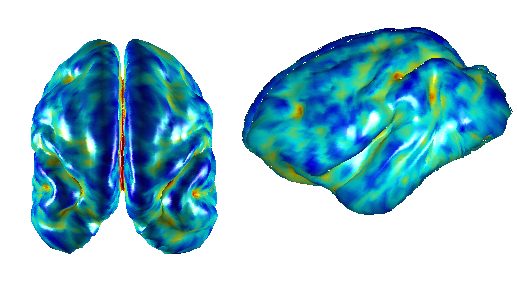
\includegraphics[width=0.5\linewidth]{Figs/mean_SI.png}
\caption{Left: Shape index for 9 monkey brains. Right: Average shape index represented on an average surface.}
\label{Fig5}
\end{figure}

Last Fig \ref{Fig5} displays shape index maps of 9 different brains and their mean on the average surface.

\bibliographystyle{plain}
\bibliography{biblio}

\end{document}
